\PassOptionsToPackage{table}{xcolor}
\documentclass{article}

\usepackage[margin=1in]{geometry}
\usepackage{amsmath}
\usepackage{graphicx}
\usepackage{subcaption}
\usepackage{float}
\usepackage{booktabs}
\usepackage{multirow}
\usepackage{xcolor}

\title{Enhancement of scale factor accuracy of modulation algorithm for a closed-loop fiber-optic gyroscope.}
\author{Sławomir Niespodziany, slawomir.niespodziany@pw.edu.pl \\
    Institute of Computer Science, Warsaw University of Technology}

\date{\today}
\begin{document}

\maketitle


\begin{abstract}
    TODO abstract
\end{abstract}

% TODO check indenteation
% TODO check formulas

\section{Motivation}
An iFOG - Interferometric Fibre Optic Gyroscope - concept is based on the Sagnac effect
    [] % http://www.orgonelab.org/EtherDrift/Post1967.pdf, http://www.orgonelab.org/EtherDrift/Post1967.pdf
Its design has already been excercised for many years. However, the limits which hold the development back are pushed forward as technology evolves, enabling for better precision, miniaturized size or lower power consumption. At the same time, the ever progressing industry finds new and more strict applications for the gyroscopes, setting the requirements bar even higher. Such context makes the already existing designs being tested and optimized in every possible aspect. This applies equally to all the optical and electro--optic componenents, the electronics and the driving software. A crucial part of the control system of an iFOG is the modulator. In a closed-loop design it is a vital element of the feedback loop. It directly affects the overall performance. It drives the optical circuit into a predefined state, in which the circuit's response can be demodulated and error signals determined. Modulator accuracy has critical impact on the resulting performance. This paper takes a closer look at the all--digital implementation of the modulator subsystem and particularily on the algorithm controlling it. Mathematical analysis is conducted to allow for pure--software optimizations in the algorithm's accuracy.

\section{Principle of operation - open--loop configuration}
A fibre--optic gyroscope utilizes Sagnac effect. A light source generates a light beam, which is ideally split in 50/50 ratio. Each half then enters a loop of relatively long fiber through each of its ends. The fiber length $L$ determines light transit time $\tau$ through it - Equation~\ref{eq:transit_time}, where $n$ is the refraction coefficient, affecting light speed in the medium.

\begin{equation}
    \tau = \frac{L}{n \cdot c}
    \label{eq:transit_time}
\end{equation}

\noindent
The halves go past each other and exit on the opposite ends of the fiber. The optical circuit is arranged, so that the two exitting beams interfere with each other and the resulting light intensity is measured at a detector. When the circuit stays at rest, the beams interfere with zero phase shift ($\Delta\phi = 0$), resulting in maximum intensity $P_0$ measured at the detector. However, when the loop rotates, the two halves travel paths of a slightly different length, resulting in non--zero phase shift. The relative phase shift at the interference point is rotation dependent and in this paper it is reffered to as the Sagnac--induced phase shift

\begin{equation}
    \Delta\phi_s = \frac{2\pi \cdot L  \cdot D \cdot n}{\lambda \cdot c} \cdot \omega
    \label{eq:phase_shift}
\end{equation}

\noindent
where $D$ - fiber loop diameter, $\omega$ - angular velocity, $\lambda$ - wavelength.

\noindent
This has been depicted in Figure~\ref{fig:fog}, where both halves enter the loop at the entry point. After the transit time they exit through the same point. However, because of the non--zero rotation, this Entry/Exit point moves, effectively shrinking one path and extending the other. The path difference is relatively small, thus it is expressed as a phase difference in wavelength domain.

\begin{figure}[h]
    \centering
    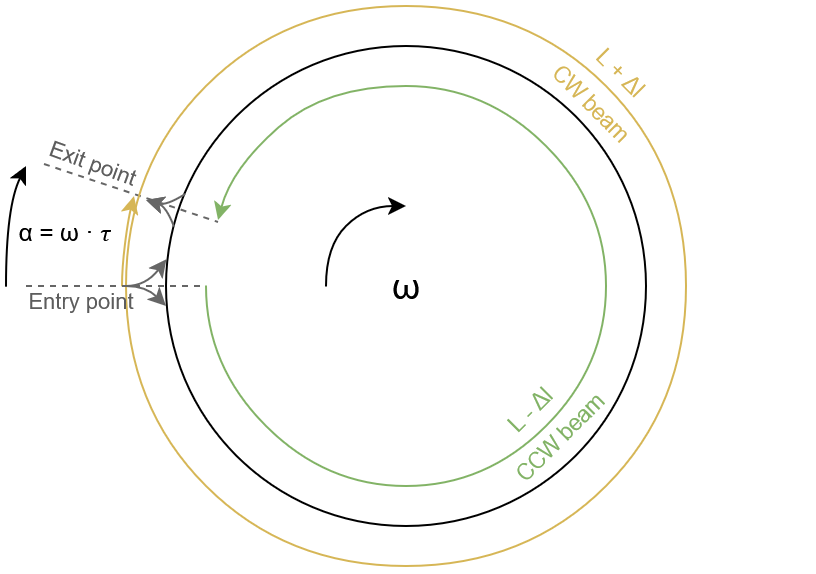
\includegraphics[width=204px]{img/fog.png}
    \caption{Two counterpropagating light beams enter the fiber loop at the \textit{Entry point}. Their phase is initially in sync. After transit time $\tau$ they exit and interfere. During that time the \textit{Entry/Exit point} moves according to the rotation rate $\omega$ (by the angle $\alpha = \omega \cdot \tau$). As a result the CW and CCW beams cover non--equal path lengths ($L\pm\Delta{}l$), which leads to a non--zero phase difference.}
    \label{fig:fog}
\end{figure}

\noindent
The formula in Equation~\ref{eq:response}, also presented in Figure~\ref{fig:response}, is the optical circuit response function.
% CITE - RESPONSE FUNCTION
It describes how the measured light intensity depends on the total phase shift of interfering light.

\begin{equation}
    P(\Delta\phi) = \frac{P_0}{2} \cdot (1 + cos(\Delta\phi))
    \label{eq:response}
\end{equation}

\begin{figure}[h]
    \centering
    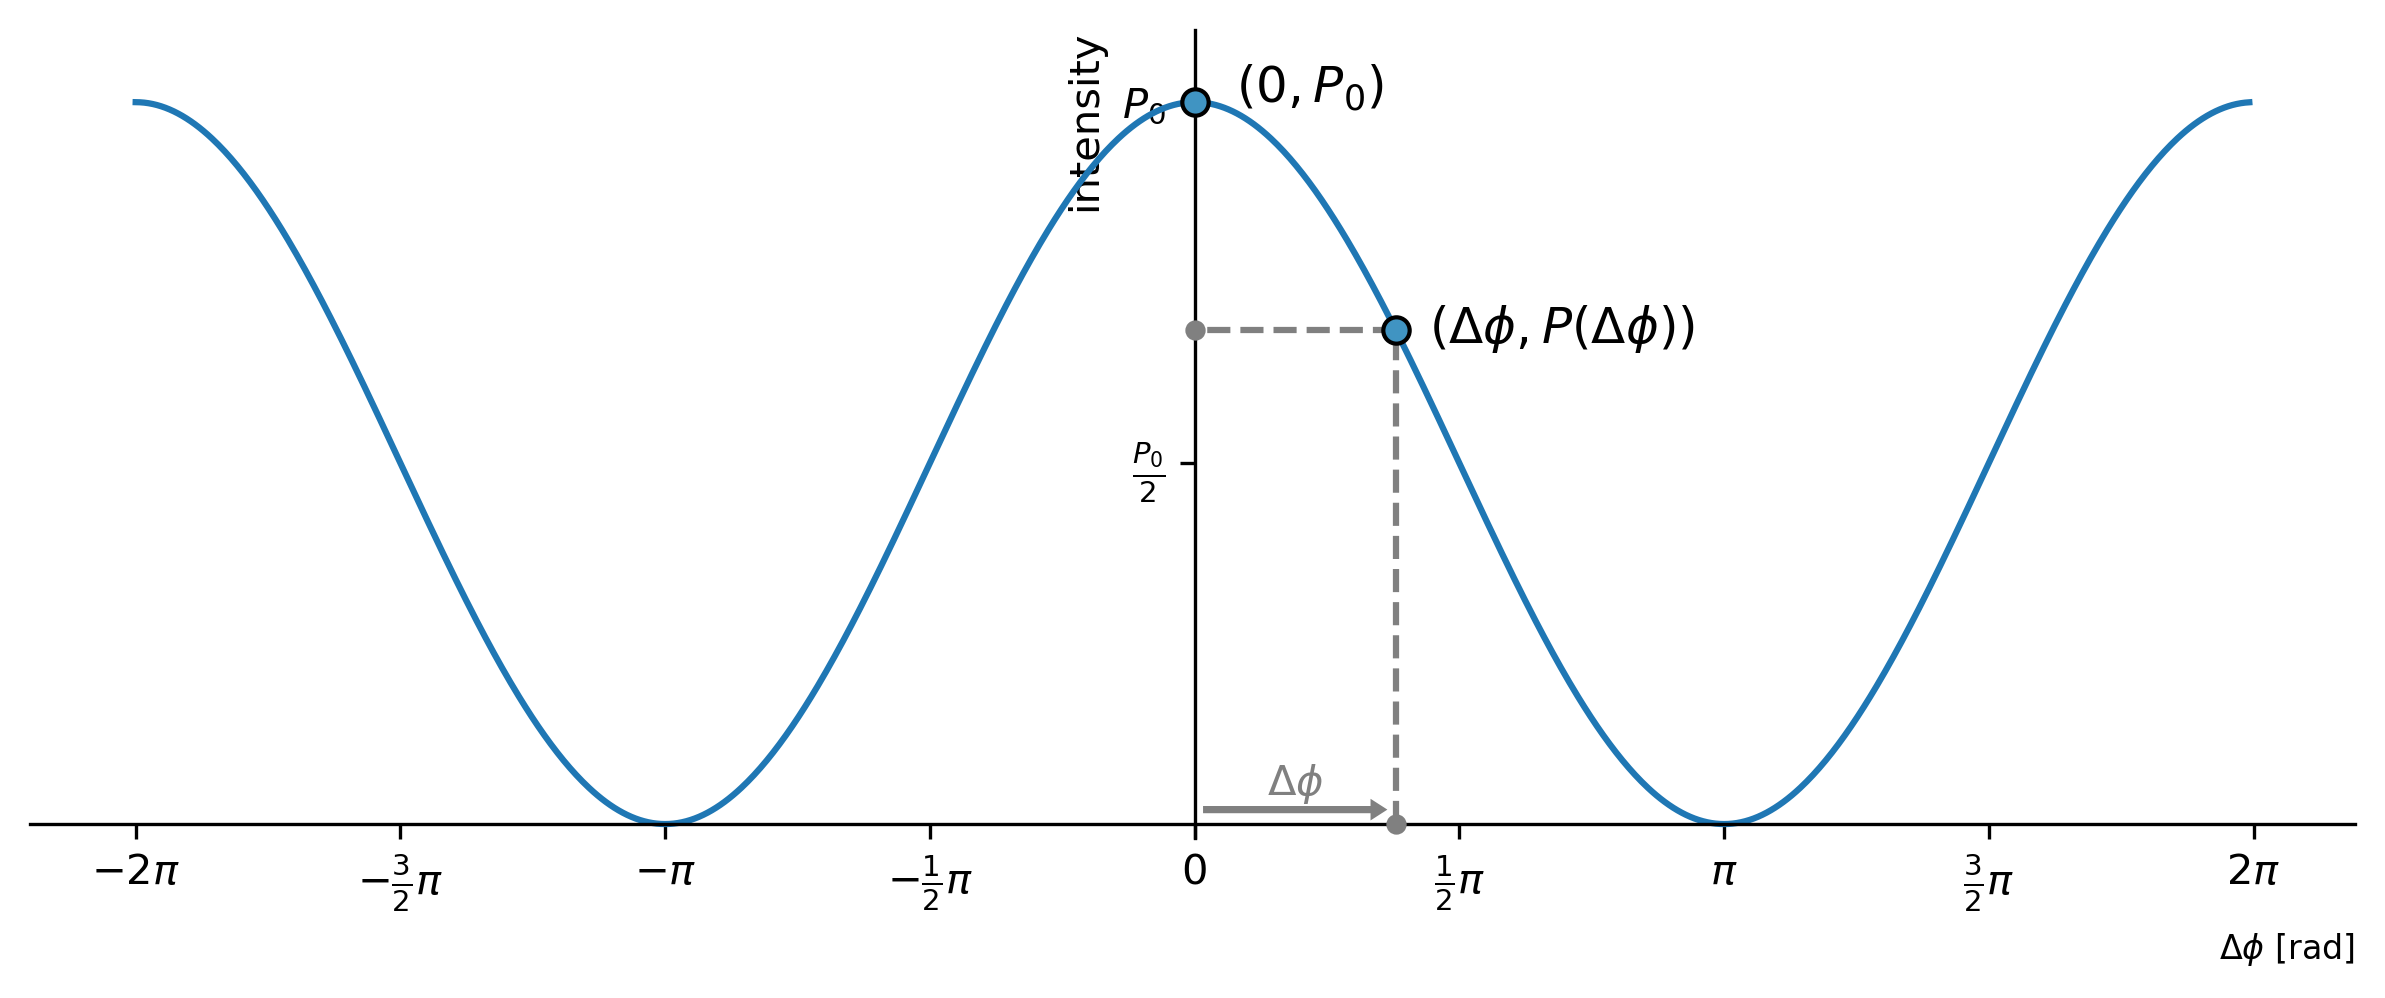
\includegraphics[width=0.75\linewidth]{img/response.png}
    \caption{Optical circuit response is a shifted cosine. The two exemplary operating points refer to the circuit being at rest, yielding the maximum possible intensity - $(0, P_0)$ - and subjected to rotation, at non--zero phase shift and decreased intensity - $(\Delta\phi, P(\Delta\phi))$.}
    \label{fig:response}
\end{figure}

\noindent
When the circuit is at rest ($\omega = 0 \rightarrow \Delta\phi = 0$), the operating point resides at peak intensity $P_0$. A non--zero rotation results in phase shift moving the operating point according to rotation rate and direction, decreasing measured intensity. Two problems are linked with this \textit{open--loop} operation.
% CITE - OPEN LOOP OPERATION
Firstly, intensity drop alone does not allow for determining rotation direction - response function is symmetrical. Secondly, in the resting region, the slope is flat, thus the sensitivity is zero. With greater rotation rate, the slope becomes more steep, reaching its maximum sensitivity in $\Delta\phi = \pm\frac{\pi}{2}$, but then decreases again. For these reasons a closed--loop configuration is superior in performance.

\section{Modulation scheme - closed--loop configuration}
In a closed--loop configuration control system biases the optical circuit sequentially in four predefined points $\Delta\phi \in \{+\frac{3}{2}\pi, -\frac{1}{2}\pi, -\frac{3}{2}\pi, +\frac{1}{2}\pi\}$, utilizing the \textit{four--step modulation}
% CITE FOUR_STEP_MODULATION
(Figure~\ref{fig:bias}). This allows for linearizing the response, keeping the circuit at maximum sensitivity and detecting rotation direction.

\begin{figure}[h]
    \centering
    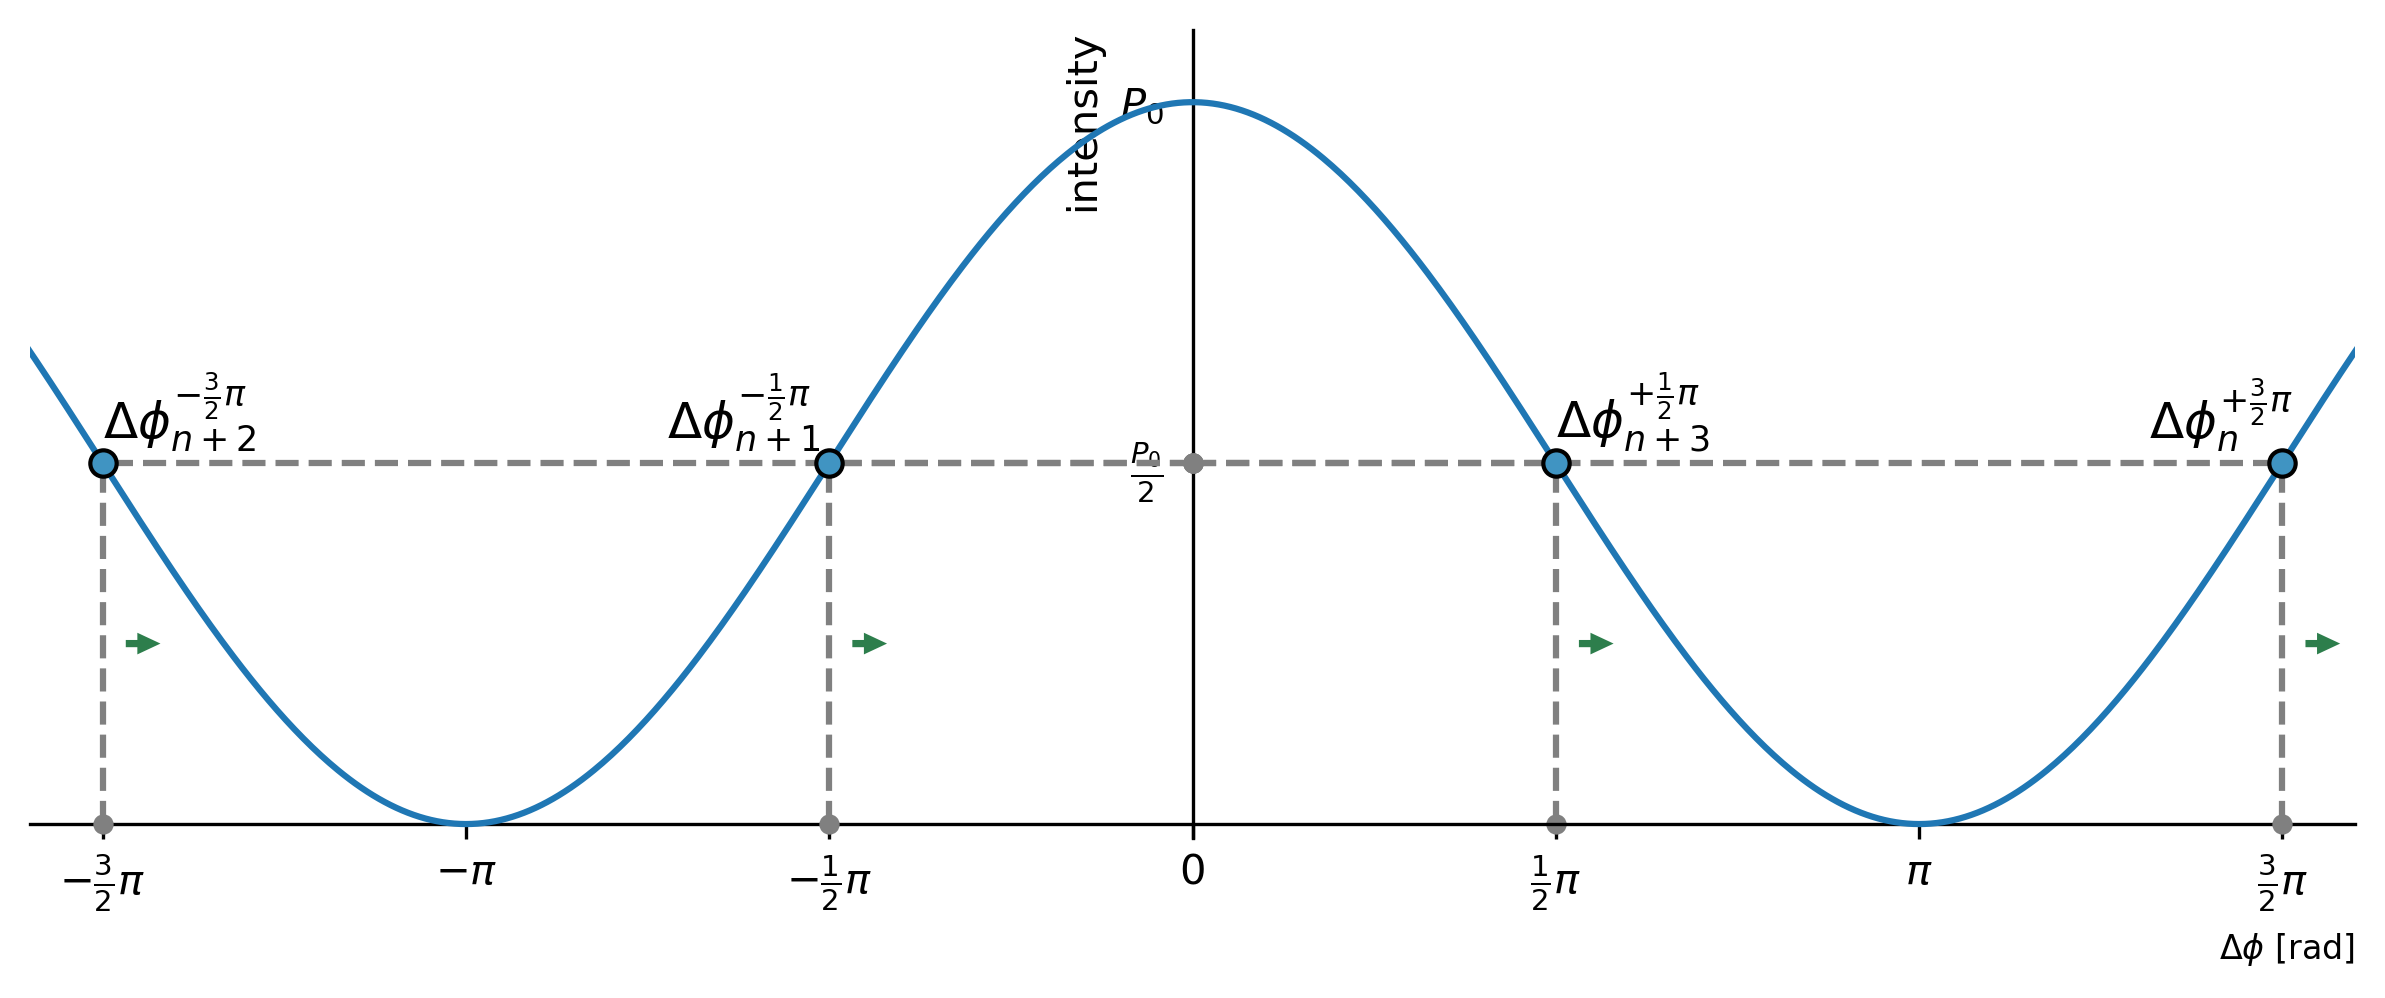
\includegraphics[width=0.75\linewidth]{img/bias.png}
    \caption{Circuit biased in four points of highest sensitivity.}
    \label{fig:bias}
\end{figure}

Compared to \textit{two--step modulation}
% CITE TWO_STEP_MODULATION
this scheme is supreme, as it allows for controlling the scale factor - a crucial parameter. Modulator injects the mentiobned phase shifts by using an electro--optic actuator placed on the fiber path. The amount of applied shift is controlled by an electronic circuit. It performs digital calculations and generates corresponding voltages via a digital--to--ananlog converter and an electronic front--end. The voltage is translated to a phase shift according to the half--wave voltage $V_\pi$, a parameter of the actuator. Additionally, each element in this pipeline is a subject to temperature drift and aging
% CITE LNB GAIN VS TEMP AND AGE
- effects which influence the total combined gain. For this reason, continous calibration is required for maintaining measurement accuracy. In short, the control algorithm needs to know where the desired bias points are in the digital domain, while they constantly drift.

Diagrams in Figure~\ref{fig:bias_errors} depict how the biased circuit responds to various conditions - misaligned scale factor and uncompensated rotation present. These errors allow the control loop for adjusting control parameters to place the points back to where they are intended and to measure the occuring rotation.

From control point of view, the combined scale factor can be reffered to as the half--wave voltage $V_{\pi}$. Even though it is only one of its components, the assumed linearity of others, makes it convenient to aggregate all into one parameter. Other, non--linear errors, such as DAC INL are out of scope of this analysis.

\begin{figure}[h]
    \centering
    \begin{subfigure}[b]{0.49\textwidth}
        \centering
        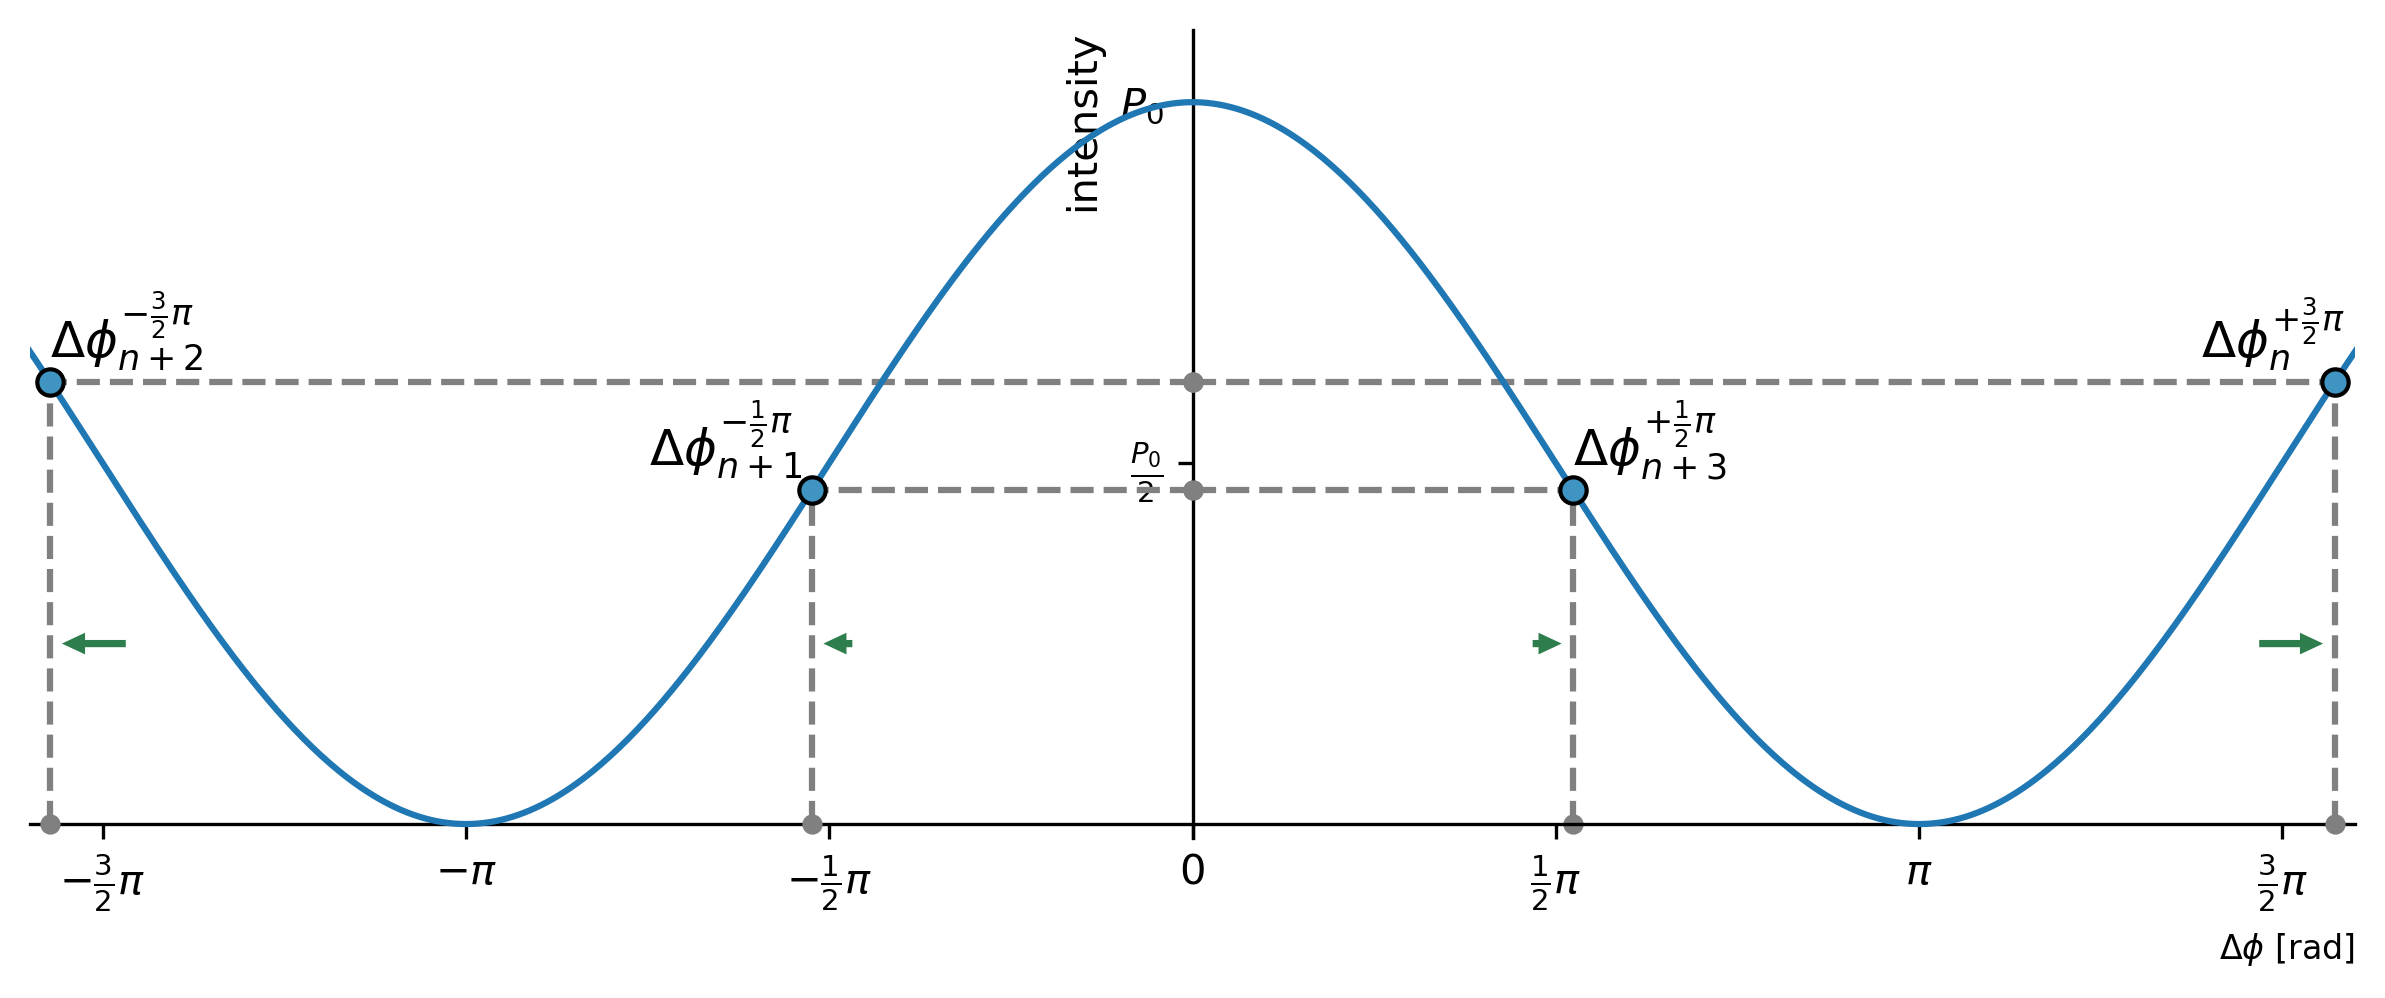
\includegraphics[width=\textwidth]{img/bias_factor_high.png}
        \caption{Scale factor too high - bias points are shifted away from zero, resulting in intensity imbalance.}
        \label{fig:bias_factor_high}
    \end{subfigure}
    \begin{subfigure}[b]{0.49\textwidth}
        \centering
        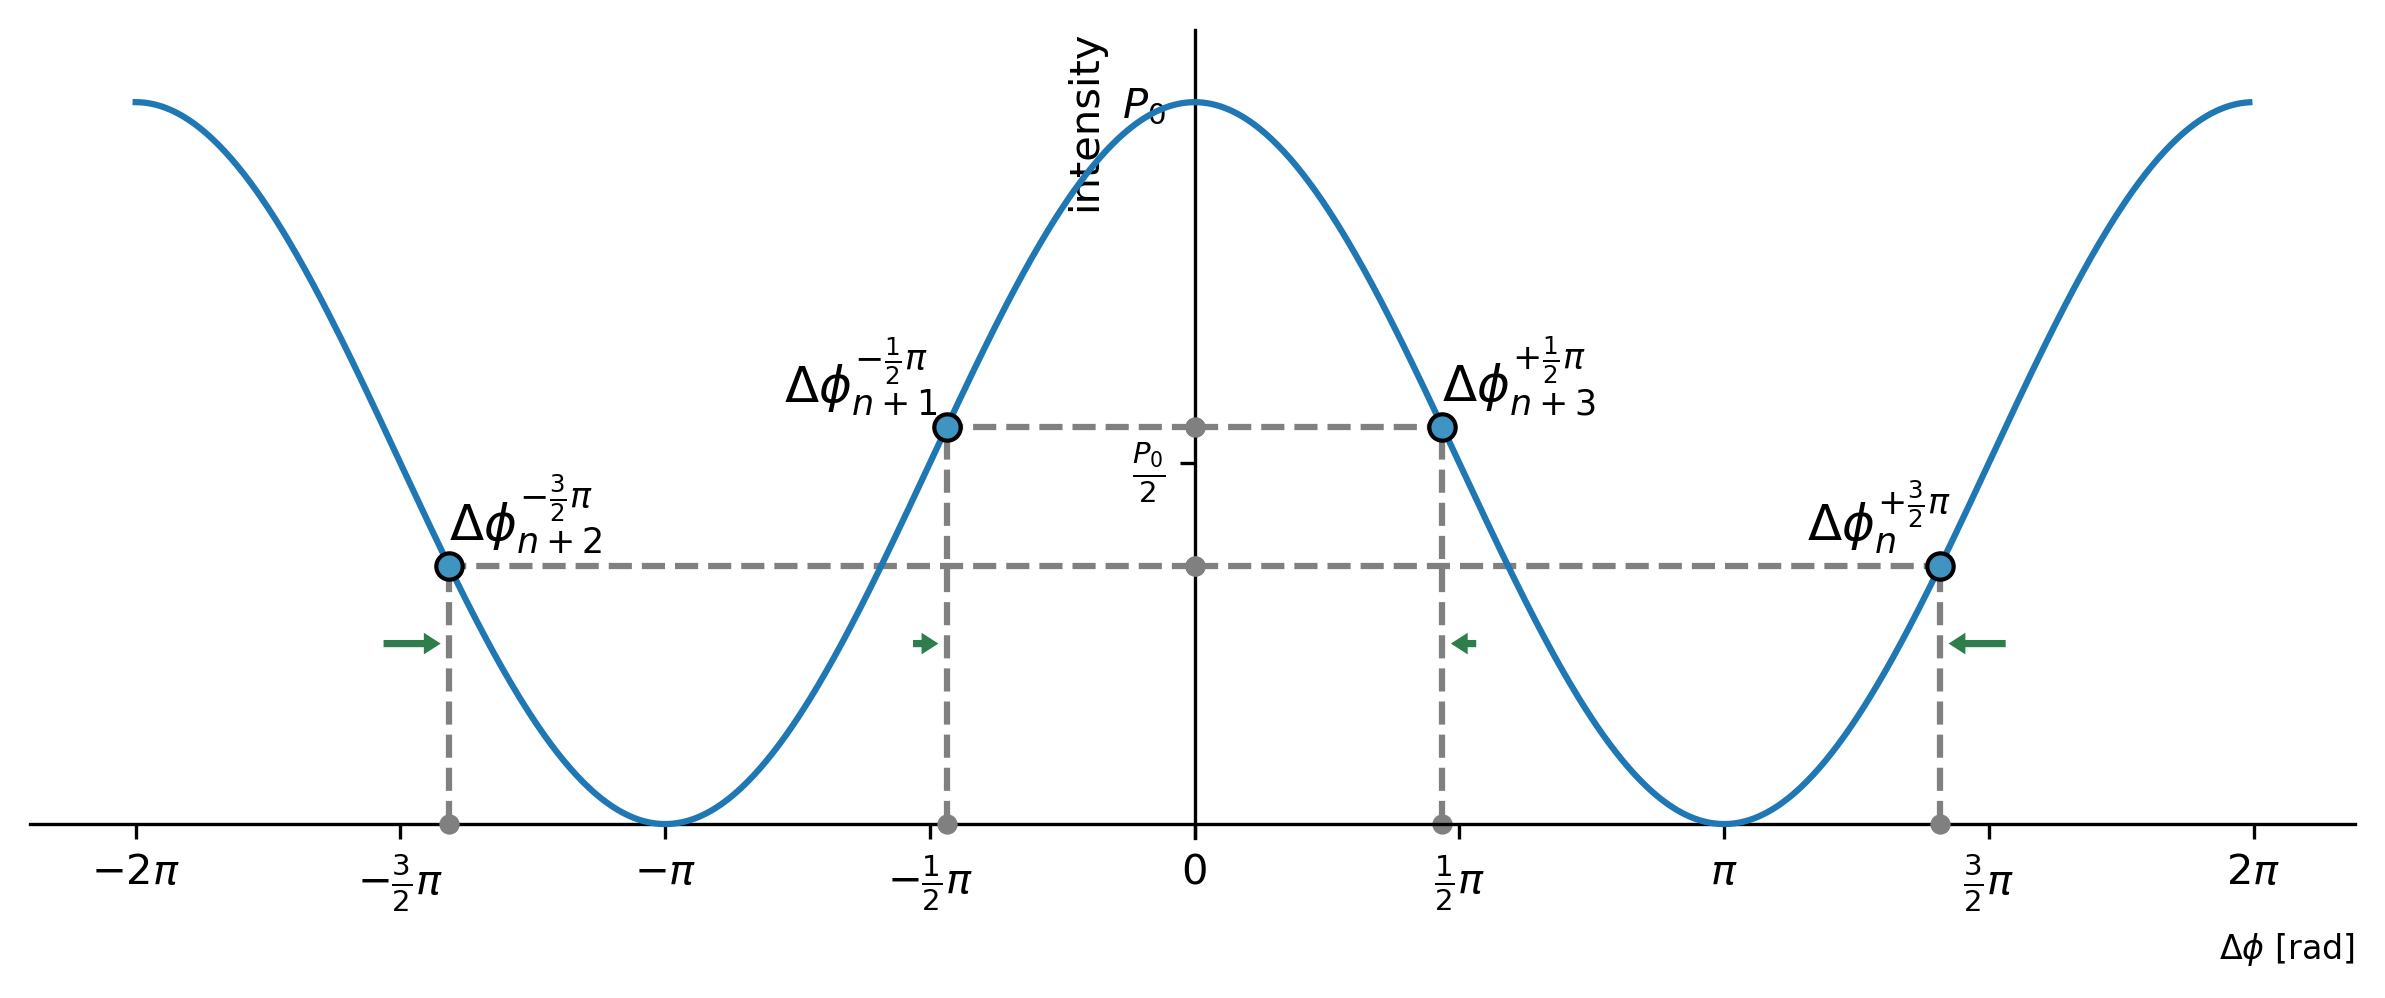
\includegraphics[width=\textwidth]{img/bias_factor_low.png}
        \caption{Scale factor too low - bias points shifted towards zero, resulting in opposite imbalance.}
        \label{fig:bias_factor_low}
    \end{subfigure}
    \begin{subfigure}[b]{0.49\textwidth}
        \centering
        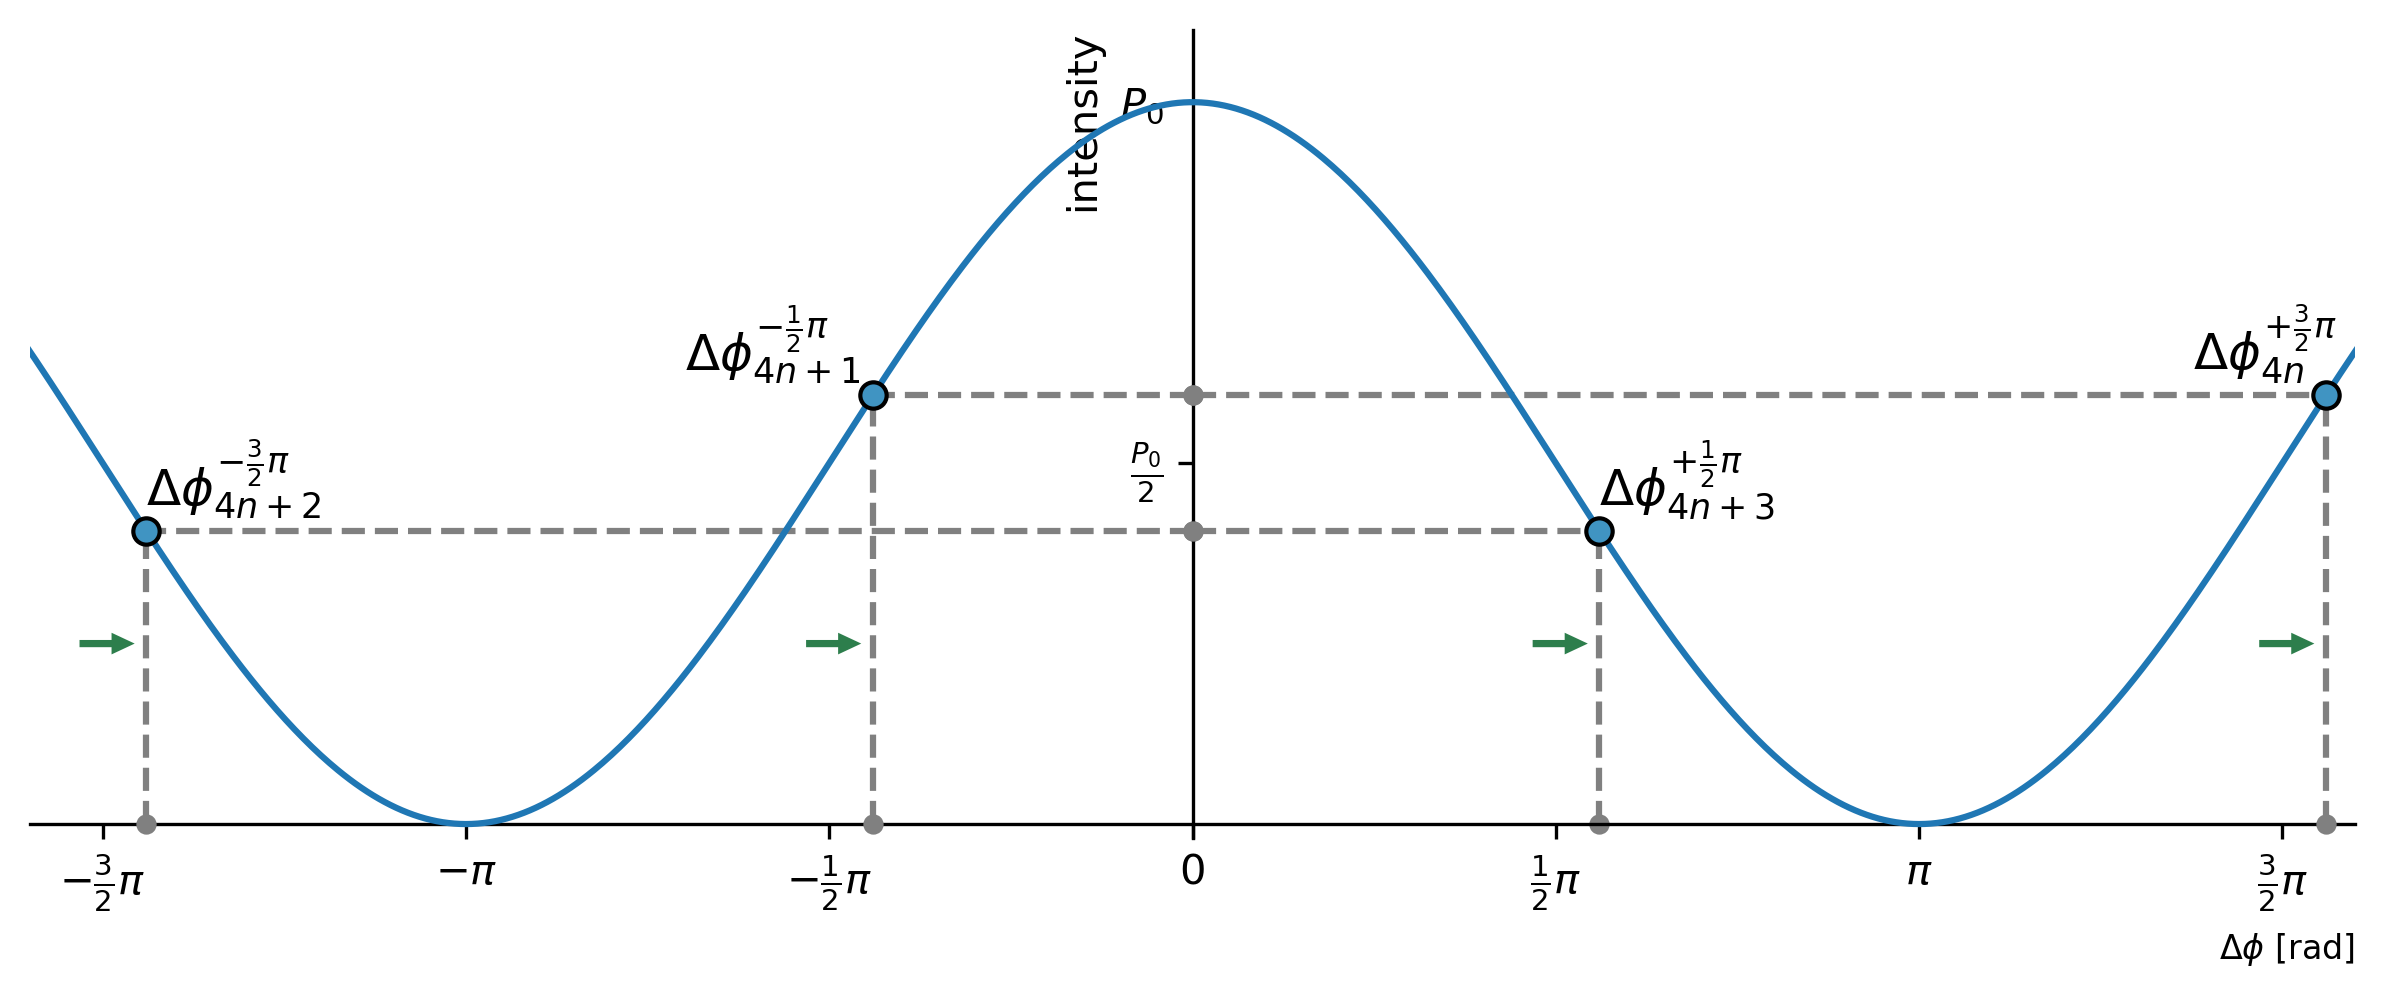
\includegraphics[width=\textwidth]{img/bias_shift_pos.png}
        \caption{Phase shift induced by positive rotation - bias points shifted right. Points $\{4n, 4n+1\}$ correspond to higher intensity than points $\{4n+2, 4n+3\}$.}
        \label{fig:bias_shift_pos}
    \end{subfigure}
    \begin{subfigure}[b]{0.49\textwidth}
        \centering
        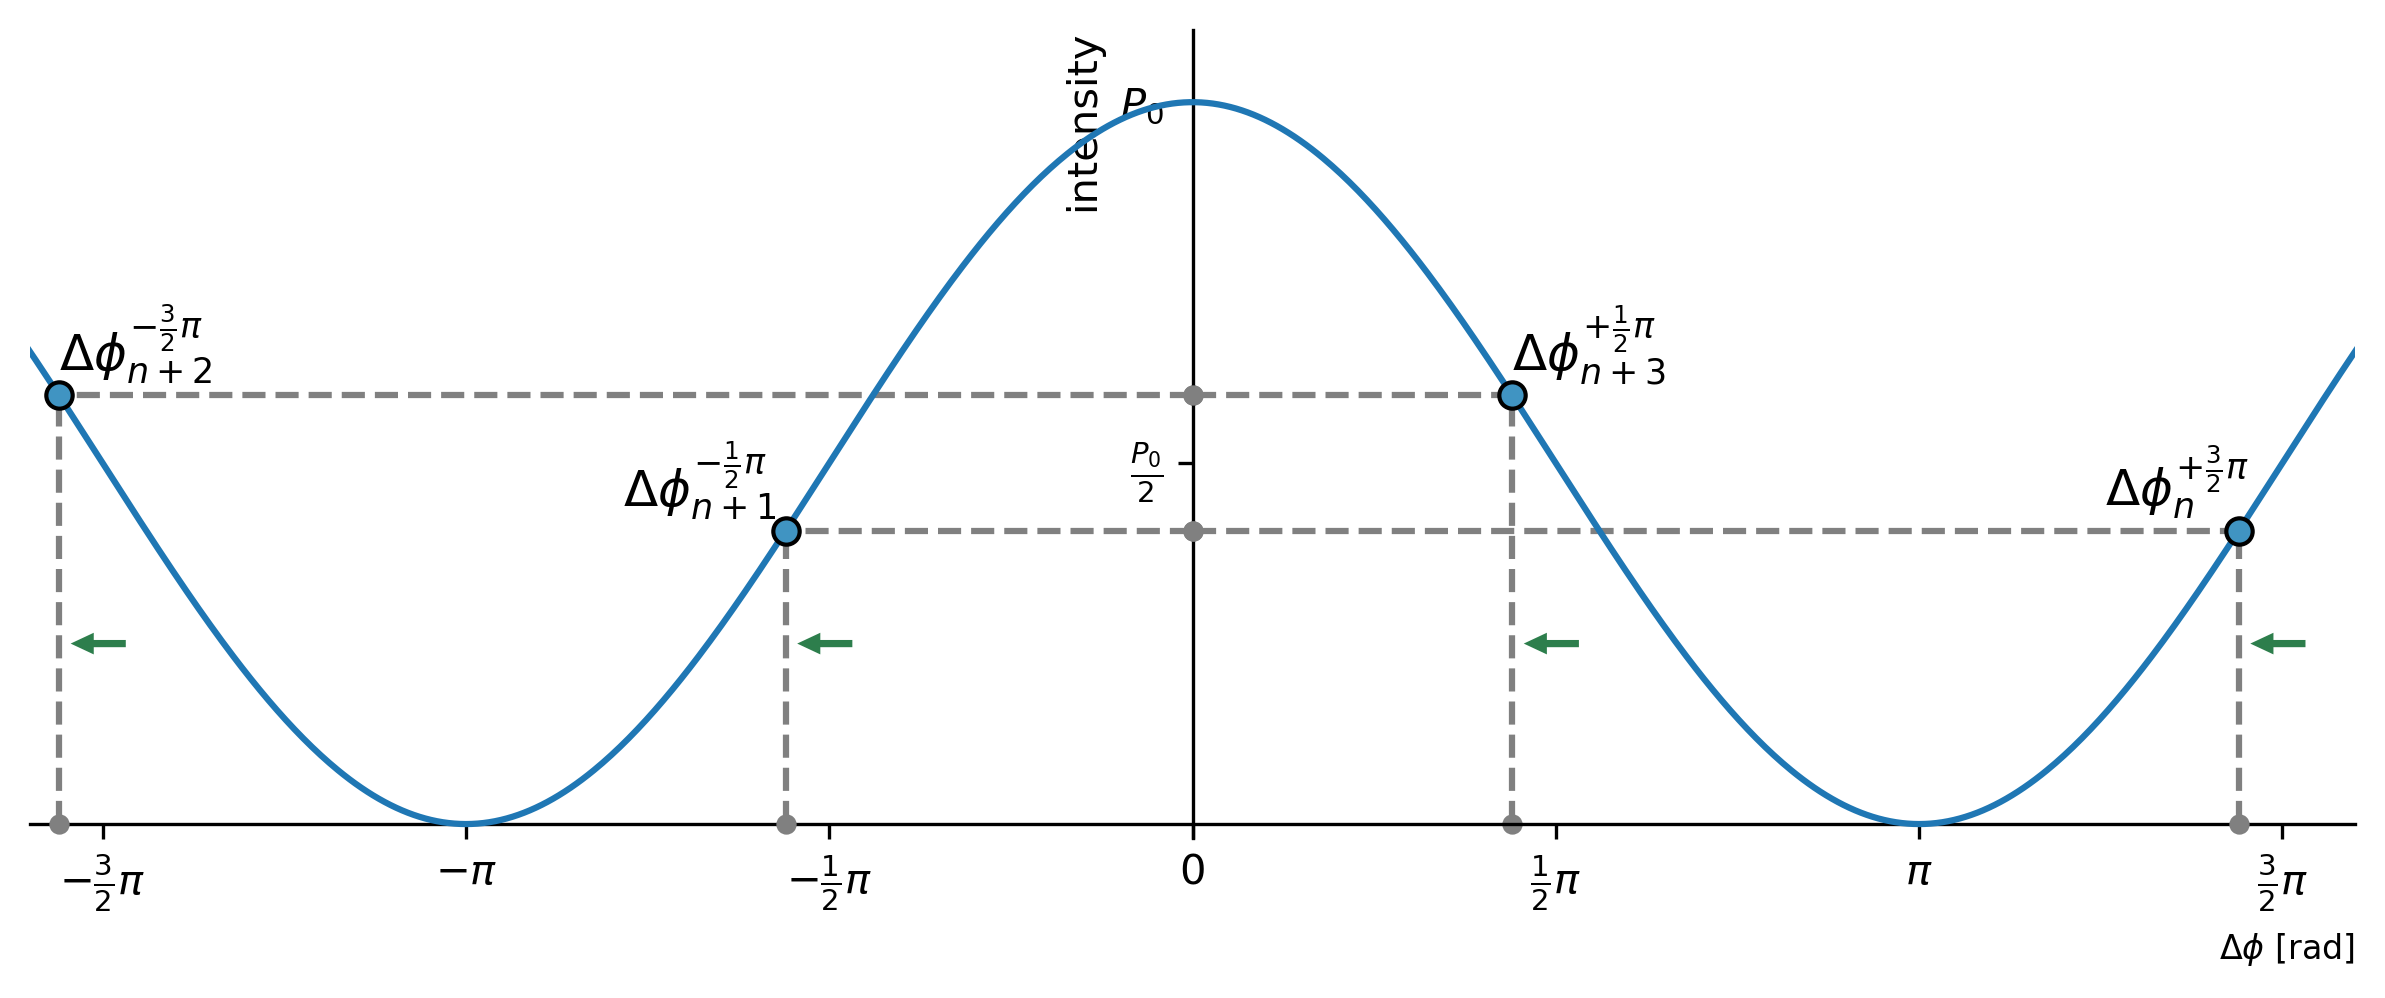
\includegraphics[width=\textwidth]{img/bias_shift_neg.png}
        \caption{Phase shift induced by negative rotation - bias points shifted left. Points $\{4n, 4n+1\}$ correspond to lower intensity than points $\{4n+2, 4n+3\}$.}
        \label{fig:bias_shift_neg}
    \end{subfigure}
    \caption{Four--step modulation allows for detection of scale factor error and Sagnac--induced phase shift.}
    \label{fig:bias_errors}
\end{figure}

Control system biases the circuit continously with the following bias point order

\begin{equation}
    \begin{split}
        \{ & \Delta\phi_{4n+0}^{+\frac{3}{2}\pi} \rightarrow (+\frac{3}{4}\pi),   \\
           & \Delta\phi_{4n+1}^{-\frac{1}{2}\pi} \rightarrow (-\frac{1}{4}\pi),   \\
           & \Delta\phi_{4n+2}^{-\frac{3}{2}\pi} \rightarrow (-\frac{3}{4}\pi),   \\
           & \Delta\phi_{4n+3}^{+\frac{1}{2}\pi} \rightarrow (+\frac{1}{4}\pi) \}
    \end{split}
    \label{eq:bias_order}
\end{equation}

\noindent
where the superscripted phase is the intended effective phase shift for the given sample.

Modulator runs with the period of half the transit time $\frac{\tau}{2}$. This allows for the effective phase shift to be a result of a relative difference between every $k$'th and $(k-2)$'th samples. For this reason the phase shift applied by the modulator for each sample can be half of the desired amplitude.
% CITE? MODULATION ALGORITHM:
Additionally, to null the effect of the rotation--induced phase shift (the Sagnac--induced phase shift), modulator adds an ever--updating ramp signal, utilizing Serrodyne modulation
% CIRE SERRODYNE MODULATION
, with the increment value of $\Delta\phi_r = -\Delta\phi_s$ - of equal amplitude, but opposite sign. This way the algorithm nulls out the Sagnac--induced shift, while knowing how much of it it has cancelled, thus knowing the exact rotation rate. In every cycle, the software monitors feedback signals and adjusts control accordingly.
% CITE MORE ALGORITHM CONTROL LOOP_CLOSED_LOOP

\section{Modulator hardware architecture}
This paper opts in for an all--digital modulator implementation. Its architecture can be designed in several ways. Firstly - a fully analog variant, while feasible, does not comply with todays standards, where information is usually processed in digital form. For integration with external systems, an analog--to--digital interface would need to be present anyway. In such case, incorporating an MCU or DSP in the processing loop brings the advantage of performing certain operations on pure data, rather than on signals carrying these data. In such context, a modern solution shall consist of a digital part for performing mathematical operations and several electronic elements for interfacing with the optical circuit - this resembles a typically implemented solution, with dedicated gain stage. Moreover, in a wolrd of \textit{software--defined}
% CITE SOFTWARE DEFINED SOLUTIONS
solutions, an architecture with the minimal amount of electronic components can also be derived. The two latter concepts are described in this section. The all--analog architecture will not be discussed.

\subsection{Dedicated gain stage}
A reasonable tradeoff between analog and digital approaches is the architecture proposed in
%CITE LEFEVRE
. It is composed of a digital part, DAC and dedicated gain stage. The configuration has been depicted in Figure~\ref{fig:dedicated_gain_stage}.

\begin{figure}[h]
    \centering
    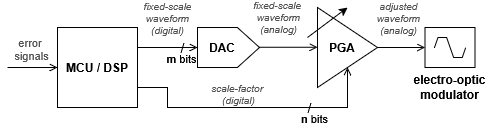
\includegraphics[height=90px]{img/dedicated_gain_stage.png}
    \caption{Modulator with a dedicated hardware gain stage. MCU/DSP outputs a fixed--scale digital waveform, which directly drives a DAC. Then, before reaching the electro--optic actuator, scale factor of the analog waveform is adjusted with a programmable gain amplifier (PGA), or a custom gain stage, resulting in adjusted--scale waveform. }
    \label{fig:dedicated_gain_stage}
\end{figure}

In this configuration DAC and PGA are driven with $n-$ and $m$--bit words. The digital nature of controlling gain stage introduces quantization noise into the control loop. However, one of the important advantages of this setup is the intrinsic separation of the modulation problem into two smaller parts - generating the waveform in fixed--scale and applying the scale factor. The two can be implemented by software without dependence on each other. On the contrary, the dedicated gain stage is a subject to interferences. It may have its own nonlinearities and introduce delay in the signal path. Most importantly, its bandwidth may be gain dependent, distorting the waveform.

% FIX FIX FIX
% Utilizing the observation, that the scale factor shall not vary by more than a few per cent during the device's lifetime, it can be assumed that if the PGA was driven by $n+1$ bits, the performance would not be affected.
% Voltage range would have to be set for the worst--case scenario plus some margin, to always be sufficient. Full scale wouldn't be used most of the time. Even if the scale factor was to drop to 50\% of the available range, which is beyond any pessimistic scenario, the overall performance would remain no worse than when using a $n$--bit control. From this an all--digital architecture can be defined.

\subsection{All-digital approach - software--defined solution}
The all--digital approach depicted in Figure~\ref{fig:all_digital} utilizes the availability and wide range of high precision digital--to--analog converters. It allows for disposing the physical gain stage, by applying scale factor digitally, prior to driving the DAC. This requires DAC reference voltage to be high enough to cover all possible ranges. This approach also introduces quantization noise. These two disadvantages, are similarily the problems of the previous solution. The main advantage this idea brings is the minimization of the amount of electronic components used. This yields less sources of potential nonlinearities and electromagnetic interference. Since the electro--optic modulator has high input impedance, the output of a voltage--DAC can be directly connected to it, omitting any buffers on the signal path. The profit resulting from less noisy electronics copensate the unavoidable DAC resolution loss - its full range may never be utilized because of the required margins. Moreover, the following sections discusses an algorithmic approach, which regains one bit of accuracy, when using the all--digital architecture.

\begin{figure}[h]
    \centering
    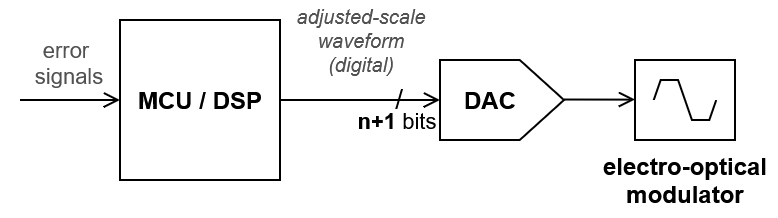
\includegraphics[height=75px]{img/all_digital.png}
    \caption{. }
    \label{fig:all_digital}
\end{figure}

Additional advantage of leaning towards the proposed architecture is, that the whole design becomes a software--defined solution. As in other fields, it brings flexibility from the R\&D process perspective. While iterating hardware design is a time--consuming process, updating software is relatively quick and cos effective. Offloating the whole problem to the software side, obviously makes teh implementation more complex, but it limits the amount of interaction at the boundary of software and hardware development. From this perspective the net workload remains at the same order of magnitude, offering slightly different, modern, approach.

\subsubsection{Voltage reference}
For an all--digital modulator an adequate reference voltage has to be set up to account for the maximum possible scale factor. From Equation~\ref{eq:bias_order} it results, that a span of $1.5\pi$ is required for biasing and additionally, the Serrodyne modulator requires a span of $2\pi$. This yields the required span of $S = 3.5\pi$. Minimum DAC reference $V_{ref}^{min}$ shall account for it with some margin $M \in [1.0; 1.1]$.

\begin{equation}
    V_{\text{ref}}^{\text{min}} = V_{\pi}^{\text{max}} \cdot S \cdot M
    \label{eq:minimum_reference_voltage}
\end{equation}

\noindent
The $V\pi^{max}$ denotes the highest expected half--wave voltage. When determining final reference voltage it is advantageous to round it up to a multiple of one of typically available chip references (Equation~\ref{eq:reference_voltage_ceil}), e.g. $K \cdot 5V$ or $K \cdot 4.096V$. It makes implementing the elctronic circuit more straightfroward. In practice, a fair compromise is to utilize the resulting voltage excess for the margin $M$, so that after adding it, the $V_{ref} \approx V_{ref}^{min}$.

\begin{equation}
    V_{\text{ref}} = \lceil V_{\text{ref}}^{\text{min}} \rceil
    \label{eq:reference_voltage_ceil}
\end{equation}

\subsubsection{Effect of the quantization error}
Usage of a DAC results in quantization error. Converter resolution and its reference voltage determine the minimal controllable voltage change as

\begin{equation}
    \Delta{}v = V_{\text{ref}} \cdot 2^{-N}
    \label{eq:dac_voltage_resolution}
\end{equation}

\noindent
In phase domain the scale factor can be controlled with the accuracy corresponding to $\Delta{}v$ relative to scale factor
% FIX FIX FIX
% Scale factor error results from the distance between its controlled and actual values. It corresponds to half of $\Delta{}v$. It can vary in time, as the actual $V_{\pi}$ may continously change over time, but rather slowly (compared to the possible modulation frequencies).

\begin{equation}
    \Delta\phi_{v} = \frac{\Delta{}v}{V_\pi}
    \label{eq:relative_scale_factor_error2}
\end{equation}

\noindent
It can vary over time, but rather slowly in the context of modulation frequency. The resulting equation depends of a few parameters, while quantization error is half of its value.

\begin{equation}
    \Delta\phi_{v} = \frac{\lceil V_{\pi}^{\text{max}} \cdot S \cdot M \rceil \cdot 2^{-N}}{V_{\pi}}
    \label{eq:total_error}
\end{equation}

\begin{equation}
    \Delta\phi_{q} = \frac{1}{2} \cdot \Delta\phi_{v}
    \label{eq:relative_scale_factor_error}
\end{equation}

\noindent
Exemplary calculation, based on real--world values yields

\begin{equation}
    \begin{split}
        \Delta\phi_{v}^{\text{ex}} & = \frac{\lceil \overbrace{4.5V}^{V_{\pi}^{\text{max}}} \cdot \overbrace{3.5}^{S} \cdot \overbrace{1.025}^{M} \rceil \cdot \overbrace{2^{-16}}^{2^{-N}} }{\underbrace{3.5V}_{V_{\pi}}} = \frac{\lceil 16.14V \rceil \cdot 2^{-16}}{3.5V} = \frac{\overbrace{16.384V}^{4 \cdot 4.096V} \cdot 2^{-16}}{3.5V} = \\
                                   & = 2^{-16} \cdot 4.68 = 2^{-16} \cdot 2^{2.23}                                                                                                                                                                                                                                                               \\
        \Delta\phi_{q}^{\text{ex}} & = \frac{1}{2} \cdot \Delta\phi_{v}^{\text{ex}} = 2^{-16} \cdot 2^{1.23}
    \end{split}
    \label{eq:error_example}
\end{equation}

\noindent
From this it is clear, that the quantization error, bound to controllable resolution can be improved by selecting a converter with greater number of bits.
However, the resolution loss will always stay at the level of over two bits. It must be noted, that most of this loss is due to the span $S$, required for proper operation of the algorithm. It is not a consequence of using the proposed all--digital architecture.

\noindent
In each of the bias points, the following drive levels are possible.

\begin{equation}
    \begin{split}
        \phi_{4n+0}^{+\frac{3}{2}\pi} & = k_{4n+0} \cdot \Delta\phi_{v} = +\frac{3}{4}\pi + \delta_{4n+0} \\
        \phi_{4n+0}^{-\frac{1}{2}\pi} & = k_{4n+1} \cdot \Delta\phi_{v} = -\frac{1}{4}\pi - \delta_{4n+1} \\
        \phi_{4n+0}^{-\frac{3}{2}\pi} & = k_{4n+2} \cdot \Delta\phi_{v} = -\frac{3}{4}\pi - \delta_{4n+2} \\
        \phi_{4n+0}^{+\frac{1}{2}\pi} & = k_{4n+3} \cdot \Delta\phi_{v} = +\frac{1}{4}\pi + \delta_{4n+3}
    \end{split}
    \label{eq:22213}
\end{equation}

\noindent
Value $k \in [-2^{N-1}, 2^{N-1}-1)$ is an integer, in range of the used DAC (of $N$ resolution). By incrementing/decrementing $k_{n}$ the error $\delta_{n}$ can be controlled with the resolution of $\Delta\phi_{v}$. However, because of the quantization error, its value can always be up to $\Delta\phi_{q}$.

% TODO number of bits n change to uppercase N (& M)
% TODO error floor
% TODO this paper does not focus on serrodyne precision, only on scale factor accuracy

\section{Precision estimation and impact}
To close the control loop, scale factor error feedback is required. It is calculated from the incident light intensity difference between two consecutive bias points in each pair. The total phase shift difference $\Delta\phi_{k}$, affecting intensity for the sample $k$, results from the current drive $\phi_k$ and the drive two points prior.

\begin{equation}
    \Delta\phi_{n} = (\phi_{n} - \phi_{n-2}) + \underbrace{\Delta\phi_{s, n} + \Delta\phi_{r, n}}_{=0}
    \label{eq:phase_shift_difference}
\end{equation}

\noindent
The values of $\Delta\phi_{s, n}$ and $\Delta\phi_{r, n}$ denote the Sagnac--induced phase shift and the nulling ramp shift, which are assumed to be zero for this analysis. By using equations \ref{eq:response} and \ref{eq:bias_order} and assuming the $cos$ function linear near the bias points (Equation~\ref{eq:cosine_linearization}), intensity values at each bias point are

\begin{equation}
    \begin{split}
        P_{4n+0}^{+\frac{3}{2}\pi} & = \frac{P_0}{2} \cdot (1 + cos(\Delta\phi_{4n+0}^{+\frac{3}{2}\pi})) = \frac{P_0}{2} \cdot (1 + cos(\phi_{4n+0}^{+\frac{3}{2}\pi} - \phi_{4n-2}^{-\frac{3}{2}\pi})) = \\
                                   & = \frac{P_0}{2} \cdot (1 + cos((\frac{3}{4}\pi + \delta_{4n+0}) - (-(\frac{3}{4}\pi + \delta_{4n-2})))) =                                                             \\
                                   & = \frac{P_0}{2} \cdot (1 + cos(\frac{3}{2}\pi + \delta_{4n+0} + \delta_{4n-2})) =                                                                                     \\
                                   & = \frac{P_0}{2} \cdot (1 + (\delta_{4n+0} + \delta_{4n-2}))                                                                                                           \\
        P_{4n+1}^{-\frac{1}{2}\pi} & = \frac{P_0}{2} \cdot (1 - (\delta_{4n+1} + \delta_{4n-1}))                                                                                                           \\
        P_{4n+2}^{-\frac{3}{2}\pi} & = \frac{P_0}{2} \cdot (1 + (\delta_{4n+2} + \delta_{4n+0}))                                                                                                           \\
        P_{4n+3}^{+\frac{1}{2}\pi} & = \frac{P_0}{2} \cdot (1 - (\delta_{4n+3} + \delta_{4n+1}))
    \end{split}
    \label{eq:incident_power}
\end{equation}

\begin{equation}
    cos(\phi_{b} + \Delta\phi) = \underbrace{cos(\phi_{b})}_{=0} + cos'(\phi_{b}) \cdot \Delta\phi = -sin(\phi_{b}) \cdot \Delta\phi \qquad \text{for } \phi_{b} \in \{+\frac{3}{2}\pi, +\frac{1}{2}\pi, -\frac{1}{2}\pi, -\frac{3}{2}\pi\}
    \label{eq:cosine_linearization}
\end{equation}

\noindent
Feedback signal can be calculated at samples $4n+1$ and $4n+3$ and yields

\begin{equation}
    \begin{split}
        e_{4n+1}^{-\frac{1}{2}\pi} & = P_{4n+1}^{-\frac{1}{2}\pi} - P_{4n+0}^{+\frac{3}{2}\pi} = -\frac{P_0}{2} \cdot (\delta_{4n+1} + \delta_{4n+0} + \delta_{4n-1} + \delta_{4n-2}) \\
        e_{4n+3}^{+\frac{1}{2}\pi} & = P_{4n+3}^{+\frac{1}{2}\pi} - P_{4n+2}^{-\frac{3}{2}\pi} = -\frac{P_0}{2} \cdot (\delta_{4n+3} + \delta_{4n+2} + \delta_{4n+1} + \delta_{4n+0}) \\
    \end{split}
    \label{eq:difference}
\end{equation}

\noindent
It can be generalized for every odd bias point, where it shall be calculated - this results from the demodulation algorithm assumptions.

\begin{equation}
    e_{2n+1} = -\frac{P_0}{2} \cdot (\underbrace{\delta_{2n+1}}_{\text{current}} + \underbrace{\delta_{2n+0} + \delta_{2n-1} + \delta_{2n-2}}_{\text{three prevoius errors}})
    \label{eq:difference_generic}
\end{equation}

\noindent
The error signal, used for control loop closure, is dependent on four recent drive values. Different weights are assigned to even and odd samples. Because the DAC can be controlled with $\Delta{}v$ resulotion, the scale factor error, and thus the occuring errors $\delta_n$ are all controllable with some minimal phase difference $\Delta\phi^{min}$ corresponding to $\Delta{}v$.

\begin{equation}
    \Delta\phi^{min} \equiv \Delta{}v
\end{equation}



\section{Algorithm design}

\subsection{Naive implementation}


\subsubsection{Number of samples considered}
Modulation algorithm serves role of a subsystem for the contol loop implemented in the device. By the fact thet the feedback signal for the scale factor control is obtained for every two bias points, as a natural consequence the feedback loop operates with such rate. This requirements falls down to the modulator. In such scenario it is tempting to implement the modulator to drive the two next bias points to obtain next feedback value. This solution is however not full (niepełny), as the feedback signal depends on the four last samples. The previous samples may act as digital noise source, disrupting the feedback signal and affecting scale factor control loop stability. A corrected solution is to account for the recent two samples drive, while calculating the next two. The total shift applied across these samples controls the feedback signal.

\subsubsection{Drive symmetry}
The intended drive values between samples $n$ and $n+2$ are symmetrical, i.e. they differ in sign, but have identical amplitude. However, for an actual signal driven with a DAC, this assumption falls short. This is due to the discrete nature of a DAC. In ideal scenario a symmetric drive would be desired, but this assumes an ideally controlled amplitude. When the amplitude is discreticized, the most bneficial solution is to utilize as much of the resolution, while keeping the drive signals relatively symmetrical as a second priority. This allows for having a $1 [lsb]$ difference in their amplitudes and thus controlling the relative difference up to a single lsb. Otherwise, the effective resolution would be lowered by one bit - the difference betweeen two effective drive values would correspond to $(k_{n} \cdot \Delta\phi_{v}) - (-k_{n} \cdot \Delta\phi_{v}) = 2\Delta\phi_{v}$ for adjacent $k_{n}$, while the DAC offers control with $\Delta\phi_{v}$ resolution.

\subsubsection{Rounding factor}
Another designing corner cut is the rounding method selection for driving discrete DAC values, while performing calculations with fractional resolution. Especially prone designs are the ones using floating point arithmetics (e.g. IEEE-754 float/double, typically used in C/C++ of programmable logic). The problem lays in the rounding direction when working with both positive and negative values (which is the case for drifing bias points both ways from zero). Mathematically this operation shall be symmetrical, however this leads to resolution loss. This is regardless whether the rounding algorithm selected is:
\begin{itemize}
    \item truncation, or rounding towards zero ($-2.4 \rightarrow -2$, $2.5 \rightarrow 2$),
    \item mathematical rounding ($2.4 \rightarrow 2$, $2.5 \rightarrow 3$),
    \item rounding away from zero ($-2.4 \rightarrow -3$, $2.4 \rightarrow 3$),
\end{itemize}

TODO check example for all three!!! TODO

\noindent
If the algorithm rounds fractional values symmetrically, it will lead to a simillar effect as in the previous section. While the effect is the same, the reason may be different, because the symmetry may also result from other factors. This case is simply worth of emphasizing, as it is expected for multiple implementations to use floating point arithmetics. This is an important nummerical issue, wspecially when performing calculations in floating point and only mapping the result to the integer, or fixed--point type required by a DAC. The below snippet shows an example.

\begin{figure}[h]
    \centering
    \begin{verbatim}
// corresponds to half-wave voltage (PI shift), in DAC units (lsb)
uint8_t scaleFactorIntended = 14u; 

int8_t dacDrive[4n+0] = round(scaleFactorDriven * 0.75) = round(10.5) = 11;
int8_t dacDrive[4n+1] = round(scaleFactorDriven * -0.25) = round(-3.5) = -4;
int8_t dacDrive[4n+2] = round(scaleFactorDriven * -0.75) = round(-10.5) = -11;
int8_t dacDrive[4n+3] = round(scaleFactorDriven * 0.75) = round(3.5) = 4;
    \end{verbatim}
    \caption{. }
    \label{fig:asdasd}
\end{figure}

\noindent
The effective drive results in an error corresponding to $((4) - (-4)) - ((-11) - (11)) = 30 \quad [\Delta\phi_{v}]$ (according to Equation~\ref{eq:difference}), while the driven scale factor indicates it shall be $28$. The

Additional problem is that this only happens at the level of least significant bits, so the only reasonable way to track this error is through nummerical analysis or simulation of the actual algorithm. It will not be visible in operation, due to the magnitude relative to the rest of the waveform.

TODO screen z SDK? TODO

\subsection{Optimal implementation}
Correct implementation accomodates for the mentioned mistakes. It controls four recent samples at all times and it selects a rounding method, which has two advantages. Firstly, it is correct in terms of modulating with the accuracy of a single lsb. Secondly, it is implementation efficient. It utilizes the property of U2 number representation, which always rounds values towards $-\inf$, resembling mathematical $floor$ operation.

TODO fixed point arithmetics TODO easily implemented in C/C++ or programmable l;ogic (ie FPGAs)

\begin{figure}[h]
    \centering
    \begin{verbatim}
// previous two bias points (4n-2, 4n-1)
// uint8_t scaleFactor[4n-2] = 13;

// int8_t dacDrive[4n-2] = (scaleFactor[4n-2] *  0x3) >> 2 = 9;
// int8_t dacDrive[4n-1] = (scaleFactor[4n-2] * -0x1) >> 2 = -4;

// current two bias points (4n+0, 4n+1)
uint8_t scaleFactorIntended[4n+0] = 14u;
uint8_t scaleFactor[4n+0] = (2 * scaleFactorIntended[4n+0]) - scaleFactor[4n-2];

int8_t dacDrive[4n+0] = (scaleFactor[4n+0] * -0x3) >> 2 = -12;
int8_t dacDrive[4n+1] = (scaleFactor[4n+0] *  0x1) >> 2 = 3;
    \end{verbatim}
    \caption{example for two of four bias points, the other two are drive in analogous way. }
    \label{fig:asdasd}
\end{figure}

In this case the effective drive corresponds to what was intended - $((3) - (-4)) - ((-12) - (9)) = 28 \quad [\Delta\phi_{v}]$

- oscilations due to wiggling regulator output, equalization required, not aviodable, as the dependence on previous points is at the physical phenomenon level
- can be controlled for each 4 steps separately, but then every second feedback signal sample is not usable

\section{Conclusions and further work}
This proposal points out some easy to make mistakes in implementing a modulator algorithm and gives a solution for solving them to reach maximum accuracy in controlling scale factor for an iFOG. Several other aspects remain undiscussed in the given analysis. In particulat, the effect of generating a ramp signal with Serrodyne modulation is a material for another paper. Further work will focus on analyzing the impact of ramp generation, the Serrodyne $2\pi$ resets and their impact on the feddback signals with non--ideal scale factor, which as discussed already, can not be determined with absolute accuracy.







% verify interpunction


% TODO \\
% Scale factor error has two sources. Primarily the algorithm needs to adjust the nummerical value precisely to control the scale factor. Error in calculating this value will directly impact the accuracy. However, even with a perfect algorithm teh quantization noise resulting from the usage of a DAC leaves some error preset at all times. While the first factor is a subject for algorithmic optimization, the second one resuts from the physical circuit impleemntation and depends on several followign parameters.

% Firstly, the relative scale factor error can be denoted as in Equation~\ref{eq:relative_scale_factor_error}.

% Voltage resolution of the used DAC results directly from the number of bits of the converter (Equation~\ref{eq:dac_voltage_resolution}).

% Substituting TODO yields the formula for relative scale factor error in a worst case scenario, when the real sclae factor remains exactly in between the two controllable, discrete phase shift values, but with the assumption, that the software has perfectly calculated the scale (no error introduced by the algorithm).

% An exemplary calculation assuming some real--world values:




% !! The closed feedback loop may regulate the controlled values - in this case the scale factor - down to a resolution which it can apply.  value that is controllable 


\begin{thebibliography}{9}
    \bibitem[Doe]{doe} \emph{First and last \LaTeX{} example.},
    John Doe 50 B.C.
\end{thebibliography}

\end{document}


% analog control https://www.mdpi.com/1424-8220/16/5/604
% complex modulator with gain amplifier: https://ieeexplore.ieee.org/stamp/stamp.jsp?arnumber=11480685